% \chapter{Scenarios}\label{ch:scenarios}

% Delete the command below to remove the hints and instructions
\showscenariosnotes{}

\section{Scenarios}
    \todoinline{
	Illustrate how your architecture fulfills the most important data flows. As a rule of thumb, focus on the scenario of the assignment. Describe the scenario in terms of architectural components using UML Sequence diagrams and further explain the most important interactions in text. Illustrating the scenarios serves as a quick validation of the completeness of
	your architecture. If you notice at this point that for some reason, certain functionality or qualities are not addressed sufficiently in your architecture, it suffices to
	document this, together with a rationale of why this is the case according to you. You do not have to further refine you architecture at this point.
    }

    This section lists which sequence diagrams belong to which scenarios:
    \begin{itemize}
        \item UC11: Sensor data being processed by the system \\
              Figure \ref{fig:seq_scenario1}

        \item UC19: Subscribing to an application \\
              Figure \ref{fig:seq_scenario2}

        \item UC12: Applications issuing actuation commands \\
              Figure \ref{fig:seq_scenario3}

        \item UC14, Av3, UC18: Sensors/actuators failing \\
              Figure \ref{fig:seq_scenario4} \\
              This scenario displays the data flow when sensors/actuators fail, causing
              \begin{itemize}
                  \item deactivation of specific applications
                  \item a redundant sensor/actuator to take over in the context of a single application
              \end{itemize}

        \item Av2: Application crash \\
              Figure \ref{fig:seq_scenario5}

        \item U2, UC4: Plugging in a new pluggable device (sensor or actuator) \\
              Figure \ref{fig:seq_scenario6}

        \item Av1, UC15: Detection and handling of communication channel failure \\
              Figure \ref{fig:seq_scenario7}

        \item UC22, U1: Upgrading an application \\
              Figure \ref{fig:seq_scenario8}

        \item UC26, UC27, UC12: Sending actuation commands via a mobile app \\
              Figure \ref{fig:seq_scenario9}
    \end{itemize}

    \begin{figure}[!htp]
    	\centering
    	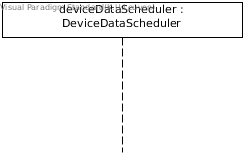
\includegraphics[width=\textwidth]{images/sequence-UC11}
    	\caption[Sensor data being processed by the system]{The pluggable device sends data to the system. The gateway receives the data and forwards it to the Online Service.
    	 The Data are saved in the Online Service in the PluggableDeviceDataDB. }\label{fig:seq_scenario1}
    \end{figure}

    \begin{figure}[!htp]
    	\centering
    	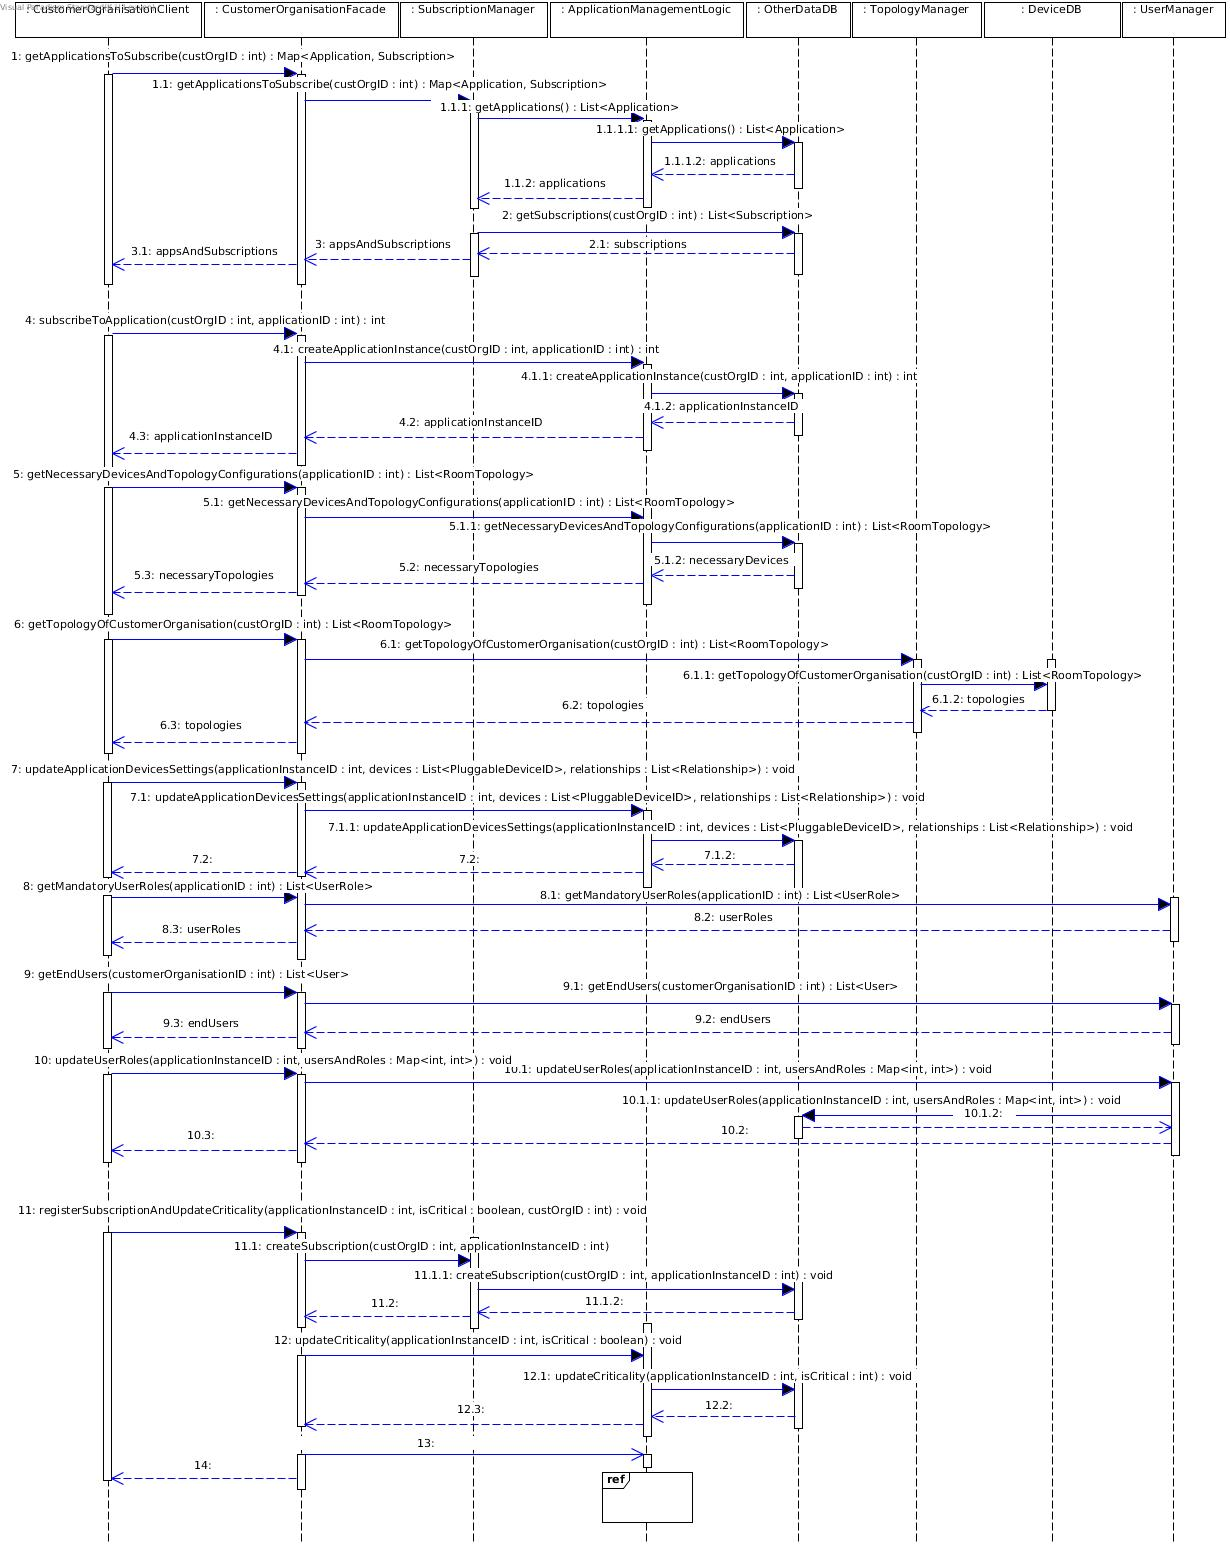
\includegraphics[width=\textwidth]{images/sequence-UC19}
    	\caption[ Subscribing to an application]{A customer organisation actor wants to subcsribe to an application. The system provides him applications to subscription
    	                        The customer organisation chooses application, sets application devices settings and user roles }\label{fig:seq_scenario2}
    \end{figure}

    \begin{figure}[!htp]
    	\centering
    	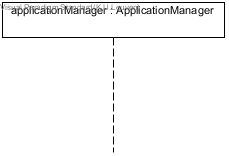
\includegraphics[width=\textwidth]{images/sequence-UC12}
    	\caption[Applications issuing actuation commands]{An application sends an actuation command to the one or more pluggable devices. The acctuation command is
    	 created according to the specific formatting syntax for the each device. }\label{fig:seq_scenario3}
    \end{figure}

    \begin{figure}[!htp]
    	\centering
    	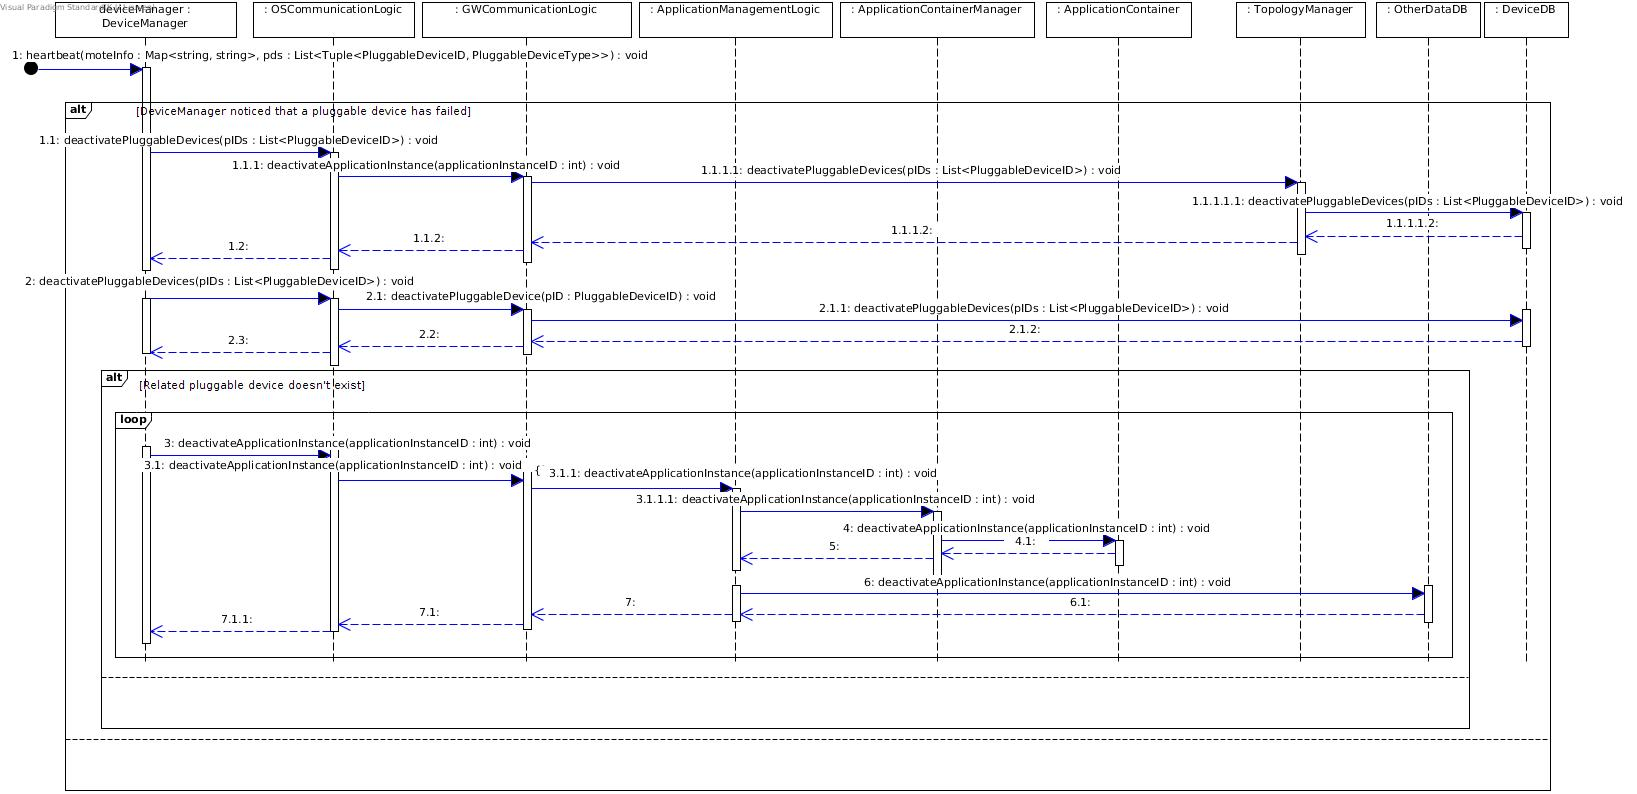
\includegraphics[width=\textwidth]{images/sequence-Av3-UC14-UC18}
    	\caption[Scenario ]{This is the flow of pluggable device failure. If there is not redundant pluggable device, then the application is deactivated.}\label{fig:seq_scenario4}
    \end{figure}

    \begin{figure}[!htp]
    	\centering
    	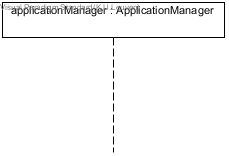
\includegraphics[width=\textwidth]{images/sequence-Av2}
    	\caption[Application crash]{ In the flow is shown failure of an application. The important part of this diagram is monitoring system, that detect failure of the application. }\label{fig:seq_scenario5}
    \end{figure}

    \begin{figure}[!htp]
    	\centering
    	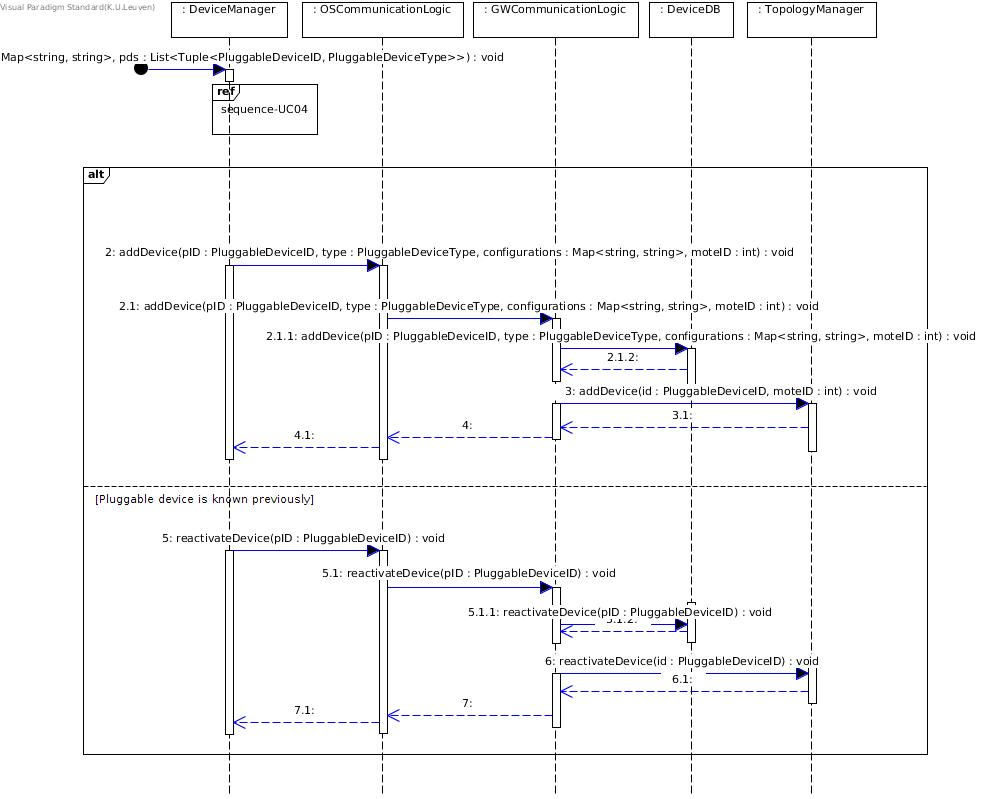
\includegraphics[width=\textwidth]{images/sequence-U2-UC4}
    	\caption[Plugging in a new pluggable device (sensor or actuator)]{ The new pluggable device is detected and save as 'inactive'. In case Pluggable device is known previously, the SloTIP reactivated the pluggable device automatically.}\label{fig:seq_scenario6}
    \end{figure}

    \begin{figure}[!htp]
    	\centering
    	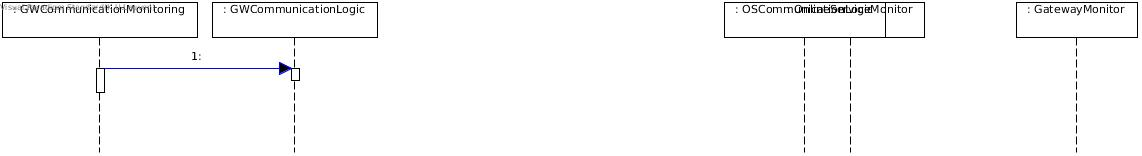
\includegraphics[width=\textwidth]{images/sequence-Av1-UC15}
    	\caption[Detection and handling of communication channel failure]{ The failure of the communicatio channel or communication component is detected with 
    	monitoring components.}\label{fig:seq_scenario7}
    \end{figure}

    \begin{figure}[h]
    	\centering
    	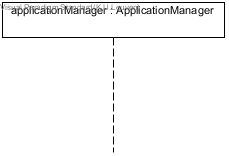
\includegraphics[width=\textwidth]{images/sequence-U1-UC22}
    	\caption[Upgrading an application]{ The application provider can upload new application or update existing.}\label{fig:seq_scenario8}
    \end{figure}

    \begin{figure}[!htp]
    	\centering
    	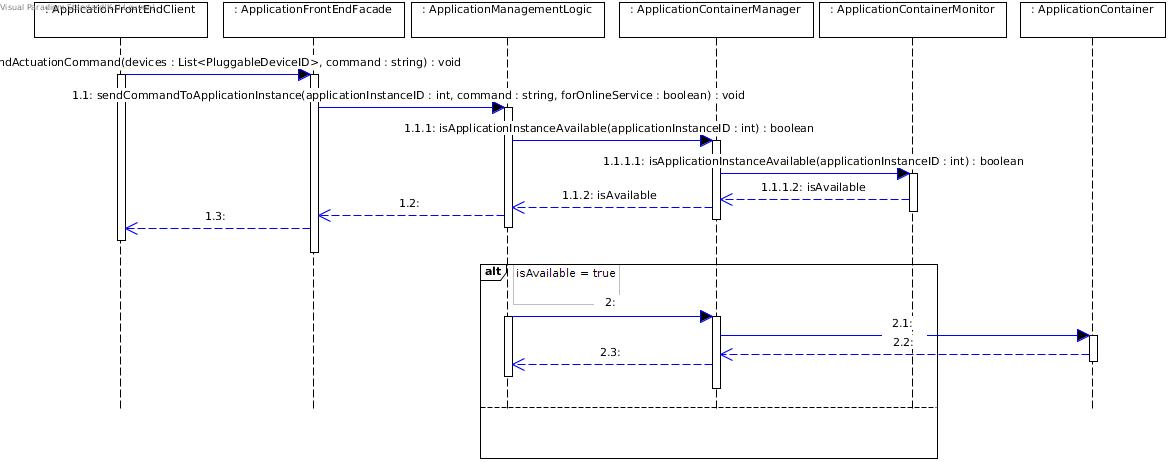
\includegraphics[width=\textwidth]{images/sequence-UC12-UC26-UC27}
    	\caption[Sending actuation commands via a mobile app]{ The application sends command from external frontend to the other parts of application. }\label{fig:seq_scenario9}
    \end{figure}
